\begin{figure}[t]
\centering
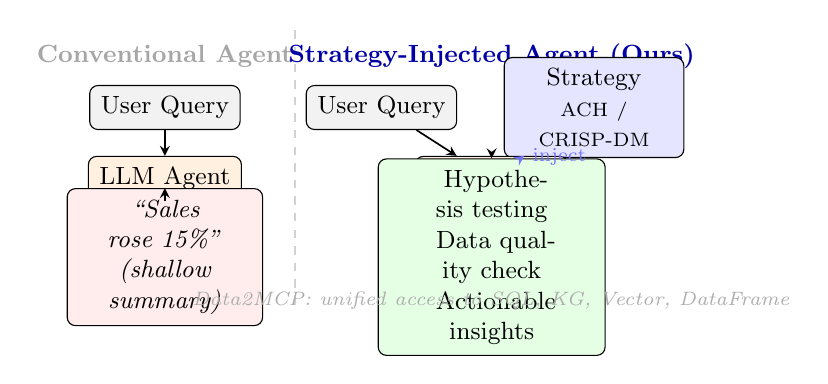
\begin{tikzpicture}[
  font=\small,
  box/.style={draw, rounded corners=3pt, minimum width=1.55cm,
              minimum height=0.52cm, align=center, inner sep=4pt},
  qbox/.style={box, fill=gray!10},
  abox/.style={box, fill=orange!12},
  sbox/.style={box, fill=blue!10},
  obox/.style={box, fill=red!7},
  gbox/.style={box, fill=green!10, text width=2.6cm},
  arr/.style={->, >=stealth, semithick},
  blkarr/.style={arr, blue!55},
]

%% ── LEFT PANEL: Without Strategy ──────────────────────────
\node[font=\small\bfseries, gray!70] at (1.4, 2.1) {Conventional Agent};

\node[qbox] (q1) at (1.4, 1.45) {User Query};
\node[abox] (a1) at (1.4, 0.55) {LLM Agent};
\node[obox, text width=2.2cm] (o1) at (1.4, -0.45)
  {\textit{``Sales rose 15\%''}\\\textit{(shallow summary)}};

\draw[arr] (q1) -- (a1);
\draw[arr] (a1) -- (o1);

%% ── DIVIDER ────────────────────────────────────────────────
\draw[gray!35, dashed, thick] (3.05, -1.05) -- (3.05, 2.45);

%% ── RIGHT PANEL: With Strategy Injection ──────────────────
\node[font=\small\bfseries, blue!65!black] at (5.55, 2.1)
  {Strategy-Injected Agent \textbf{(Ours)}};

\node[qbox]  (q2) at (4.15, 1.45) {User Query};
\node[sbox, text width=2.0cm]  (s2) at (6.85, 1.45)
  {Strategy\\{\scriptsize ACH / CRISP-DM}};
\node[abox]  (a2) at (5.55, 0.55) {LLM Agent};
\node[gbox]  (o2) at (5.55, -0.45)
  {$\checkmark$~Hypothesis testing\\
   $\checkmark$~Data quality check\\
   $\checkmark$~Actionable insights};

\draw[arr]    (q2) -- (a2);
\draw[blkarr] (s2) -- (a2)
  node[midway, right, font=\scriptsize, blue!55] {inject};
\draw[arr]    (a2) -- (o2);

%% ── BOTTOM NOTE ────────────────────────────────────────────
\node[font=\scriptsize, gray!65] at (5.55, -1.0)
  {\textit{Data2MCP: unified access to SQL, KG, Vector, DataFrame}};

\end{tikzpicture}
\caption{Strategy injection transforms LLM agents from shallow data
  porters into structured expert analysts. Data2MCP provides unified
  multi-source retrieval as the underlying infrastructure.}
\label{fig:motivation}
\end{figure}
